% For BRIGFOS, max size is 60cm wide x 150cm high. Use A1 portrait.
%
% Note: a0 is 119 x 85
%       a1 is  84 x 60 (84.1 x 59.4)
%       a2 is  60 x 42
%       a3 is  42 x 30
% Default mode is landscape, which is what we want, however dvips and
% a0poster do not quite do the right thing, so we end up with text in
% landscape style (wide and short) down a portrait page (narrow and
% long). Printing this onto the a0 printer chops the right hand edge.
% However, 'psnup' can save the day, reorienting the text so that the
% poster prints lengthways down an a0 portrait bounding box.
%
% 'psnup -w85cm -h119cm -f poster_from_dvips.ps poster_in_landscape.ps'
% 'psnup -w60cm -h84cm -f poster_from_dvips.ps poster_in_portrait.ps'

\documentclass[a1,portrait]{a0poster}
    \usepackage{pst-node,amssymb}
    \usepackage[T1]{fontenc}
    \usepackage[utf8]{inputenc}
    \usepackage[dvipsnames]{xcolor}
    \usepackage{mdframed}
    
    % You might find the 'draft' option to a0 poster useful if you have
    % lots of graphics, because they can take some time to process and
    % display. (\documentclass[a0,draft]{a0poster})

    \renewcommand{\d}{\mathrm{d}}
    \newcommand{\sgn}[1]{\mathop{\mathrm{sgn}}#1}
    \newcommand{\bu}{\textcolor{DarkBlue}{\mathbf{u}}}
    \newcommand{\bI}{{\mathbf{I}}}
    \newcommand{\bsig}{\textcolor{DarkBlue}{\boldsymbol{\sigma}}}
    \newcommand{\bx}{\mathbf{x}}
    \newcommand{\br}{\mathbf{r}}
    \newcommand{\ds}{\mathrm{d}s}
    \newcommand{\taud}{\ensuremath{\textcolor{Red}{\tau_d}}}
    \newcommand{\taur}{\ensuremath{\textcolor{Red}{\tau_r}}}
    \newcommand{\bbeta}{\ensuremath{\textcolor{Red}{\beta}}}
    \newcommand{\ie}{\textit{i.e.}}
    \setcounter{secnumdepth}{0}
    \newcommand{\comment}[1]{}
        \newcommand{\twopartdef}[4]
        {	\left\{
                \begin{array}{ll}
                    #1 & \mbox{if } #2 \\
                    #3 & \mbox{if } #4
                \end{array}
            \right.}
        \newcommand{\threepartdef}[6]
        {	\left\{
                \begin{array}{ll}
                    #1 & \mbox{if } #2 \\
                    #3 & \mbox{if } #4 \\
                    #5 & \mbox{if } #6
                \end{array}
            \right.}

    % The textpos package is necessary to position textblocks at arbitary
    % places on the page.
    \usepackage[absolute]{textpos}

    % Graphics to include graphics. Times is nice on posters, but you
    % might want to switch it off and go for CMR fonts.
    \usepackage[final]{graphics}
    \usepackage{wrapfig,helvet}
    \usepackage{amsmath}
    \usepackage[T1]{fontenc}
    
    %\usepackage{graphicx,wrapfig,lipsum}

    % These colours are tried and tested for titles and headers. Don't
    % over use color!
    \usepackage{color}
    \definecolor{DarkBlue}{rgb}{0.1,0.1,0.5}
    \definecolor{Red}{rgb}{0.9,0.0,0.1}
    \definecolor{headingcol}{rgb}{0.5,0.7,1}
    \definecolor{dgreen}{rgb}{0.1,0.7,0.1}
    \definecolor{dbrown}{rgb}{0.5,0.2,0.2}

    %\definecolor{boxcol}{rgb}{0.3,0.8,0.1}

    % see documentation for a0poster class for the size options here
    \let\Textsize\normalsize
    \def\Head#1{\noindent\hbox to \hsize{\hfil{\LARGE\color{DarkBlue}\sf #1}}\bigskip}
    \def\LHead#1{\noindent{\LARGE\color{DarkBlue}\sf #1}\bigskip}
    \def\Subhead#1{\noindent{\large\color{DarkBlue}\sf #1}\bigskip}
    \def\Title#1{\noindent{\VeryHuge\color{Red}\bf\sf #1}}

    \TPGrid[40mm,40mm]{15}{12}  % 2 cols of width 7 plus 1 gap width 1

    \parindent=0pt
    \parskip=0.5\baselineskip

    \makeatletter				%Needed to include code in main file
    \renewcommand\@maketitle{%
    \null					%Sets position marker
    {
    \color{headingcol}\sffamily\Huge	%Set title font and colour
    \@title \par}%
    \vskip 0.6em%
    {
    \color{white}\sffamily\Large		%Set author font and colour
    \lineskip .5em%
    \begin{tabular}[t]{l}%
    \@author
    \end{tabular}\par}%
    \vskip 1cm
    \par
    }
    \makeatother

 \begin{document}

    \title{Fej\'er's Theorem for Fourier Series}

    \author{\LARGE{Department of Mathematics}\\ \large{Anmol Aggarwal, Yohance Osborne, An\dj ela Markovi\'c,} \\ \large{Thevin Degamboda, Tinashe Dingwiza }}

    %----------------------------------------------------------------------%
    %           Title bar: across all 14 columns                           %
    %----------------------------------------------------------------------%
    \begin{textblock}{15}(0,0)
    \vspace*{-120mm}\hspace*{-50mm}\textcolor{black}{\rule{700mm}{93mm}}\\[-5mm]
    \vspace*{-33mm}\hspace*{-42mm}%
    \scalebox{0.5}{\includegraphics{ucl_bar_black_taller.eps}}   
    \begin{minipage}{594mm} %a1		%Minipage for title contents
    \vspace{-8.0cm}
    %\vspace{-14.1cm}
    \maketitle
    \pagestyle{empty}
    \thispagestyle{empty}
    \end{minipage}
    \end{textblock}
    \begin{textblock}{7}(0,1.4)
    \LHead{\textbf{Introduction}}

    \resizebox{\textwidth}{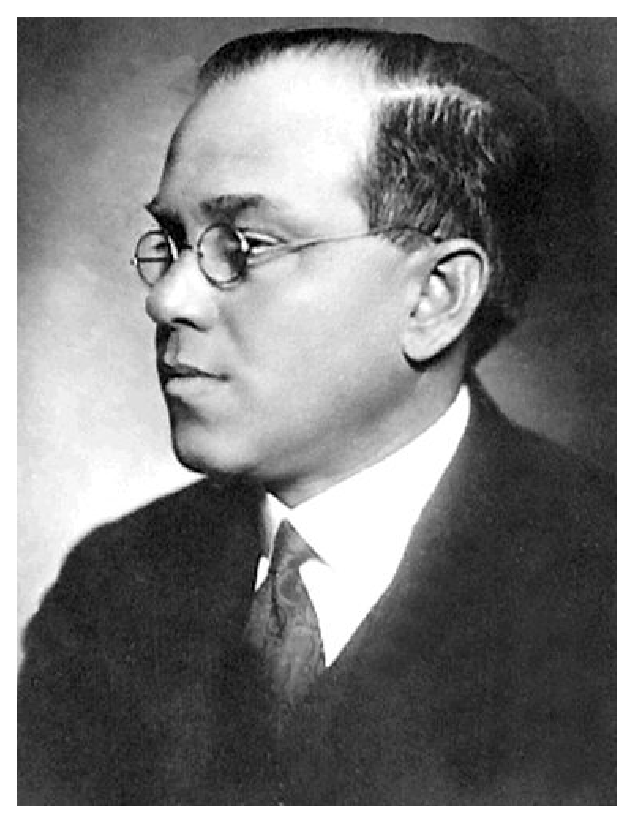
\includegraphics{fejer_lipot.eps}}
    \quad  \quad \quad \hspace*{26mm} Lip\'ot Fej\'er
    \end{textblock}

    \begin{textblock}{3.8}(3.2,1.82)
    \sf
    On the 9th of February 1880, Lip\'ot F\'ejer was born as Leopold Weiss in P\'ecs, Hungary. Around 1900, he abandoned his Germanic name in favor of a Hungarian equivalent so as to express his solidarity with Hungarian culture. Remarkably, at the age of 19 years, he proved what is now called \emph{Fej\'er's Theorem} which may be used to approximate continuous, periodic functions of one variable defined over the real numbers $\mathbb{R}$.   
    \bigskip

    \end{textblock}
    %---------------------------------------------------------------------
    \begin{textblock}{7}(0,4.15)
    \bigskip
    \hrule
    \LHead{\textbf{Definitions}}\\
    \sf \vspace{-2mm}
    Let $f$ be a locally integrable, $2\pi$-periodic function over $\mathbb{R}$.
    
    \begin{itemize}
    
    \item \textbf{Uniform Convergence}: We say that a sequence of functions $\{f_n(x)\}_{n \in\mathbb{N}}$ converges uniformly to $f$ on $[-\pi,\pi]$ if $$\lim_{n\to \infty}\left( \sup_{x\in [-\pi,\pi]}|f_{n}(x)-f(x)|\right)=0.$$ 
    \item \textbf{Fourier Coefficient $\hat{f}_k$}: Corresponding to a given integer $k$, this is a number given by
    $\hat{f}_k=\frac{1}{2\pi}\int_0^{2\pi}e^{-ikt}f(t)\text{dt}$.
    \item \textbf{Fourier Series $N$-th Partial Sum}: Given a natural number $N\geq 0$ and $x$ in the interval $[-\pi,\pi]$, this is the finite sum  $S_N(x)=\sum_{k=-N}^{N} \hat{f}_k e^{ikx}$.
    \item \textbf{$n$-th Ces\'aro average}: For any non-negative integer $n$, this is the average of the first $n+1$ partial sums $\{S_N(x)\}_{N=0}^{n}$. We denote it by $\sigma_n(x)=\frac{1}{n+1}\sum_{N=0}^nS_N(x)$.
    \end{itemize}
    \bigskip
    \hrule
    \end{textblock}

    %-----------------------------------------------------------------------%
    \begin{textblock}{7}(0,7.80)
    \LHead{\textbf{Fej\'er's Theorem}}
    
    %\Subhead{Fej\'er's Theorem}\\
    \sf
    \begin{mdframed}[linewidth = 1.5mm,linecolor = Red]
    \begin{flushleft}\hspace{5mm}
    If $f:[-\pi,\pi] \to \mathbb{C}$ is continuous at $x\in [-\pi,\pi]$
    and $f$ is \\ \hspace{5mm} Riemann integrable, then:
    $$ \sigma_n(x) \text{ converges to } f(x) \ \text{as} \  n \to \infty.$$
    \hspace{6mm} Furthermore, if $f$ is continuous, then: $$ \sigma_n \text{ converges to } f \ \text{uniformly on} \ [-\pi,\pi].$$
    \end{flushleft}
    \end{mdframed}

The first part of the theorem gives conditions which ensure that the sequence of Ces\'aro averages give good approximations of the value of the function $f$ wherever it is continuous. The final result of the theorem follows quite naturally if $f$ is continuous everywhere on its domain. 
    \end{textblock}

    \begin{textblock}{7}(0,10.68)
    \Subhead{Consequences} \vspace*{-5mm} 
    \sf \\ While Fej\'er's theorem has uses in advanced topics, such as Functional Analysis (see [4]), here three relatively elementary consequences are shared:
    \begin{itemize}

    \item If $f:[-\pi,\pi] \to \mathbb{C}$ is continuous, then there exists a sequence of trigonometric polynomials which converge uniformly to $f$ on $[-\pi,\pi].$ An example of a sequence of trigonometric\\ polynomials would be $\{S_N(x)\}_{N=0}^{\infty}$. \vspace{4mm}
    \\
    \end{itemize}
    \end{textblock}

    \begin{textblock}{7}(8,1.4)
    \sf
    
    \begin{itemize}
    \item If $f,g:[-\pi,\pi] \to \mathbb{C}$ are continuous and $$\int_0^{2\pi}e^{-ikt}f(t)dt=\int_0^{2\pi}e^{-ikt}g(t)dt$$ for all $k \in \mathbb{Z}$, then $f\equiv g$. In other words, any two continuous functions which have identical Fourier coefficients, describe the same function. 
    \item Fej\'er's theorem can be used to derive \emph{Weierstrass' approximation theorem} for continuous functions on $[-\pi,\pi]$, which states that there exists a sequence of polynomials which converge uniformly to $f$.
    \end{itemize}
    \bigskip
    \hrule
    \end{textblock}
 
    %---------------------------------------------------------------------
    \begin{textblock}{7}(8,3.75)
    \LHead{\textbf{Example}}\\
    \sf
    Consider the function: \textcolor{red}{$$ h(x) = \frac{\pi}{2} -  |x| \quad \quad x\in [-\pi, \pi].$$}We may express the $N$-th partial sum of the Fourier series for $h$ and the associated $n$-th Ces\'aro average as follows:
    \textcolor{blue}{$$ S_N(x) = \sum_{k=0}^{N} \frac{4\cos[(2k+1)x]}{\pi(2k+1)^2}, $$}
    \textcolor{blue}{$$ \sigma_n(x) = \frac{1}{2\pi}\int_{-\pi}^{\pi} \left(\frac{\pi}{2} - |t| \right)\frac{1}{n+1}\left(\frac{\sin[(n+1)\frac{(x-t)}{2}]}{\sin(\frac{x-t}{2})}\right)^2 dt. $$}
    \\
Since $h$ is continuous on $[-\pi, \pi]$, we can apply Fej\'er's theorem to deduce that
    $$ \sigma_n \text{ converges to } h \ \text{uniformly as} \  n \to \infty.$$
    \vspace{-2.6em}
    \begin{center}
    \resizebox{0.99\textwidth}{!}{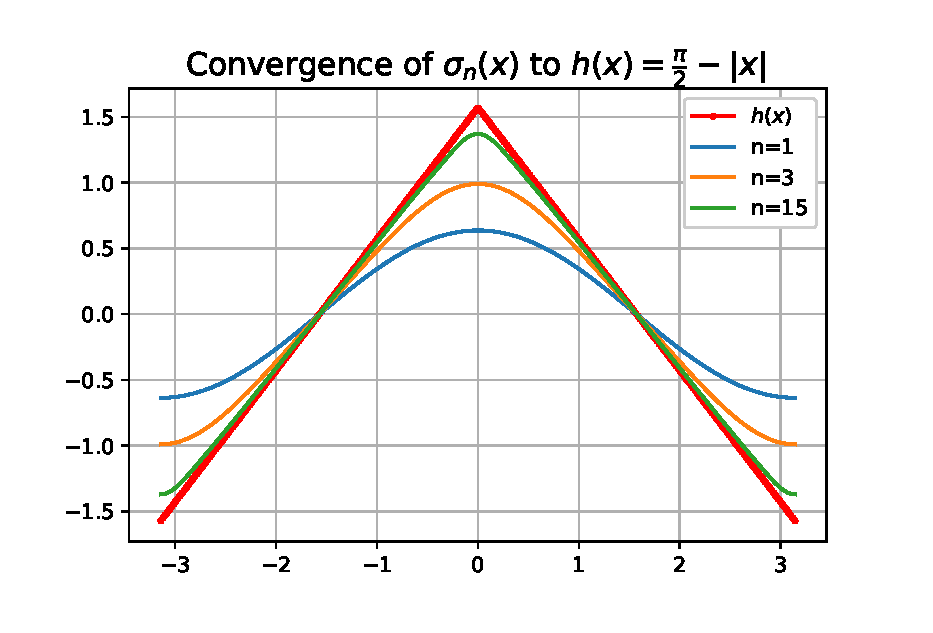
\includegraphics{graph.eps}}
    \end{center}
    \vspace{-1.6em}
    This is an illustration of uniform convergence as it shows how $\sigma_n$ better approximates $h$, over all of $[-\pi,\pi]$, as $n$ is increased.    \vspace{0mm}
    \hrule
    \end{textblock}


    \begin{textblock}{7}(8,10.10)
        
        \Subhead{Acknowledgement}
        \sf \vspace*{-10mm}
        
        This poster summarizes the second-year project which was \ undertaken in June 2018. We would like to give special thanks to Prof Alex Sobolev and Prof Michael Singer for all their help.
        \bigskip
        \hrule
    \end{textblock}

    \begin{textblock}{7}(8,11.0)%\rule{\textwidth}{0.1mm}
    \Subhead{References}

    \vspace*{-11mm}
    {\sf \footnotesize
        \begin{enumerate}
        \item[{[1]}] K\"orner, T. (1988), 'Proof of Fej\'er's theorem', 'Introduction', and 'The circle T' \\ in \textit{Fourier Analysis}. Cambridge: Cambridge University Press.
        \item[{[2]}] \text{Haggstrom, P.} (2016),  \textit{The nitty gritty of Fej\'er's  Theorem}
        \item[{[3]}] \text{Krishnapur, M.} (2017), \textit{Topics in Analysis} (pp. 1-6)
        \item[{[4]}] \text{Crioranescu I. & Lizama C.} (1997), \textit{Some Applications of Fejer's Theorem to Operator Cosine Functions in Banach Spaces} in \textit{Volume 125 Proceedings of the American Mathematical Society.}
        \end{enumerate}
    }
    \end{textblock}

\end{document}
